\documentclass[a4paper,twocolumn]{article}
\usepackage[english]{babel}
\usepackage[T1]{fontenc}
\usepackage[utf8]{inputenc}
\usepackage{lmodern}
\usepackage{setspace}
\usepackage{graphicx}

\renewcommand{\baselinestretch}{1.3}

\title{Legal basis for replacing handwritten signatures with open electronic signature software}
\author{Jakub Ďuraš, P. J. Safarik University}

\begin{document}

{\setstretch{1.0}
    \maketitle
}

\section*{Introduction}

We are usually used to signing of paper documents.
How easy it is if we want to sign some documents without meeting with another party in person?
Do we print the documents from their electronic form only because we need to sign them? There is an alternative in the form of electronic signatures.
We would like to explore on what legal ground we can create software utilizing them and what if we also want to make it a part of the open-source movement.

Unless specified otherwise, we are considering law applicable locally in the Slovak Republic (SR).
Its law is greatly influenced by the European Union (EU), being its member since 2004, and therefore, we can assume this is at least partially applicable outside of the SR.

\section{Signatures}

Essential part of the written legally binding documents, signatures are permanently affixed to the document and are supposed to uniquely identify the person and its deliberate, informed consent.
As can be seen in the Slovak Civil Code, "A written legal act is valid if signed by the acting person;" \cite{1}.
Law often explicitly requires signatures and further clarifies their expected use.
For example, when selling an enterprise, the contract is required in written form, with attested signatures of the seller and the buyer \cite{2}.

Signature is considered an "attested signature"\footnote{Translation from "osvedčený podpis" as used in the Slovak law.} if it is verified by the authorized third party.
Such process, known as legalization, is regulated by the law and its purpose is to form the basis for the exercise of legal rights \cite{3}.

With regards to electronic signatures, law within the EU used to differ, with one applicable in the SR being now repealed "Zákon č. 215/2002 Z.z.".

\section{EU Regulation eIDAS}

With the intent to stimulate digital growth by building trust, the EU established regulation on electronic identification and trust services for electronic transactions in the internal market (eIDAS).
It applies from 1st of July 2016, caused the local law to be repealed, and regulates, among other things, electronic signatures and its more advanced forms.

\begin{figure}[ht]
    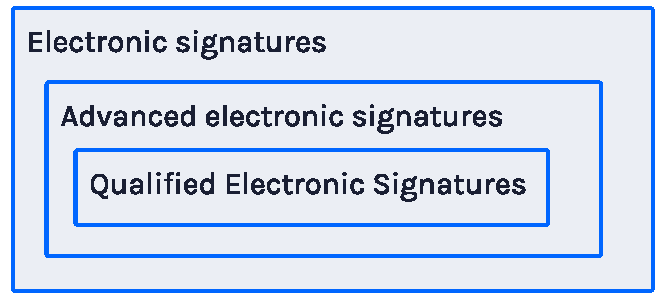
\includegraphics[width=\linewidth]{../paper/figures/electronic-advanced-qualified}
    \caption{The relation between electronic, advanced, and qualified signatures.}
    \centering
\end{figure}

In general, electronic signature can be represented in different ways (e.g. as an image, text or other data attached to the document) and it can not be denied in legal proceedings just because it is in the electronic form \cite{4}.

Advanced electronic signatures are a subset of electronic signatures that have to uniquely link and identify the signature author, be created in a way that is possible only by them, and any changes to the signed document have to be detectable \cite{5}.
From the technical point of view, standards PAdES, XAdES, and CAdES specified by the ETSI comply with these requirements.

Qualified electronic signatures (QES) are a subset of advanced electronic signatures with more specific requirements that can be found in the Annex 1 of the eIDAS regulation\footnote{Available at https://eur-lex.europa.eu/legal-content/EN/TXT/HTML/?uri=CELEX:32014R0910\#d1e32-111-1}.
In more practical terms, such advanced electronic signatures are created with a qualified device, certificate, and using a qualified trust service. Qualified in this case means authorized for such use by the legal authorities that maintain publicly accessible, transparent list.

The qualified electronic signature has the legal effect of the handwritten signature \cite{4} or attested handwritten signature in the SR specifically.

Such terminology is used only when considering natural person. Legal entities are able to use "electronic seals", which are, from the technical point of view and for our purposes, almost identical.

\section{Software copyright}

Computer programs and associated materials shoule be protected under copyright as literary works, and protected authors should be able to authorize or prohibit certain acts \cite{6}.

Such right can be exercised, as far as we are concerned, to license the software under either proprietary or open-source license.
Proprietary meaning under the exclusive legal right of the author with source code being typically also confidential and distributed as a paid product.
Open-source meaning having its source code freely available, usually also distributed for free, and without any liability (the software is provided "as is").

Motivations to license the software under an open-source license can vary, and so do such licenses.
While a proprietary license is usually made specifically for that entity and its interests, open-source licenses tend to be reused between different authors.
This means consumers of the software can quickly recognize their rights and responsibilities if they decide to use, modify, or distribute the software.
In general, we can classify the open-source licenses into two categories: permissive and copyleft.

Copyleft license, in general, requires the user to publish the modified work under the compatible (free) license.
By doing that, it forces users to extend the rights they have received onto others and, in turn, somehow limit potential use in software licensed under a different license.
Popular example of license like that is the GNU General Public License (GPL) and its derivatives like GNU Lesser GPL (LGPL) or GNU Affero GPL (AGPL).

\begin{figure*}[ht!]
    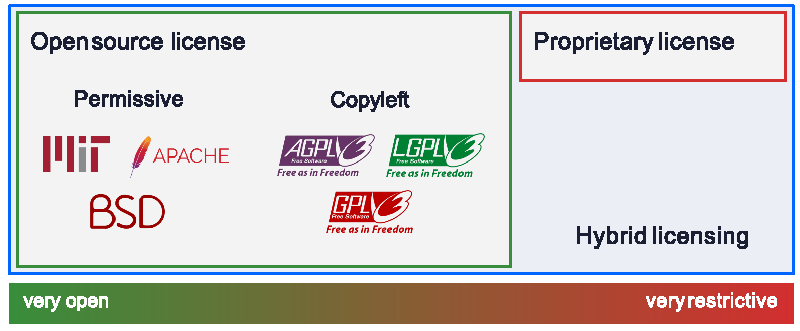
\includegraphics[width=\linewidth]{../paper/figures/license-comparison}
    \caption{Classification and comparison of software licensing models.}
    \centering
\end{figure*}

Permissive license, on the other hand, does not have such requirement in place and is more suitable for potential commercialization.
They typically allow commercial use, modifications, distribution, or sublicensing as long as the author is not held liable, and the original copyright and license are distributed with the software.
Often used permissive licenses are MIT License, Apache License, or BSD License.

It is not uncommon to see hybrid licensing - licensing under more than one license, with one being typically open-source and one proprietary.
In this scenario, users can choose which license they want to use based on their needs.

As we have already mentioned, software licenses can influence whether and how it can be used as a part of different software.
Both when we are using someone else's software and when someone else is using our software.
Generally speaking, the more restrictive the license is, the higher the probability it will prevent adoption for legal reasons.

\begin{figure}[ht]
    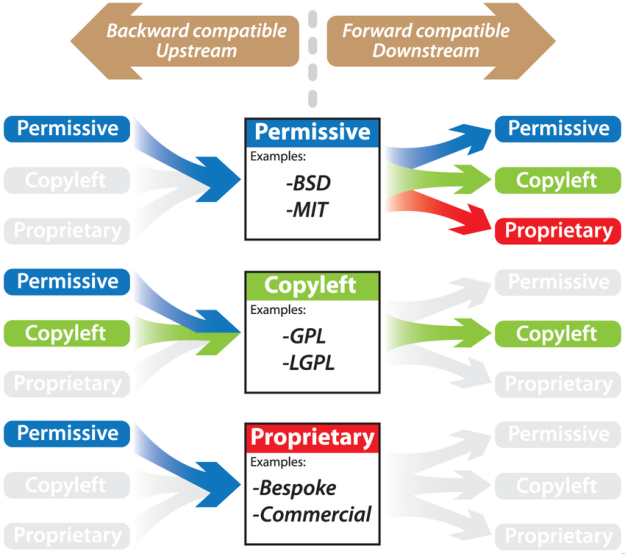
\includegraphics[width=\linewidth]{../paper/figures/license-compatibility}
    \caption{Schematic representation of license directionality \cite{7}.}
    \centering
\end{figure}

Various possible combinations can be seen in Figure 3, where greyed out options mean such combination is not possible unless a separate licensing agreement is reached with the copyright owner.

\section*{Conclusion}

Overall, electronic signatures are supposed to be, within the EU, interoperable and transparent alternative to hand-written signatures.

Utilizing open-source software is possible, provided we are mindful of the license.
Likewise, choosing the proper license can help with adoption.

\onecolumn{
    \begin{thebibliography}{9}

    \bibitem{1}
    \emph{Zákon č. 40/1964 Zb. občiansky zákonník, § 40 ods. 3}

    \bibitem{2}
    \emph{Zákon č. 513/1991 Zb. obchodný zákonník, § 476 ods. 2}

    \bibitem{3}
    \emph{Zákon č. 323/1992 Zb. notársky poriadok, § 56 ods. 1}

    \bibitem{4}
    \emph{Regulation (EU) No 910/2014, Article 25}

    \bibitem{5}
    \emph{Regulation (EU) No 910/2014, Article 26}

    \bibitem{6}
    \emph{Directive 2009/24/EC of the European Parliament and of the Council of 23 April 2009 on the legal protection of computer programs}

    %  ------
    % Article
    %  ------
    \bibitem{7}
    MORIN, A., et al. 2012. A Quick Guide to Software Licensing for the Scientist-Programmer. In: \emph{PLoS computational biology} [online]. Volume 8, issue 7 [cit. 2020-01-27]. Available at: https://journals.plos.org/ploscompbiol/article?id=10.1371/journal.pcbi.1002598

    \end{thebibliography}
}


\end{document}
